\scanpage{13}
\uline{Questions sur courbes elliptiques} sur $\overline{\mathbf Q}$.

Soit $C$ une telle courbe, $G$ son groupe de Galois motivique [$G\unsure{\simeq|\equiv}\mathrm{GL}(2,\mathbf Q)$ ou $G=\prod_{K/\mathbf Q}G_m$, $K$ le corps de multiplication complexe]. Soit $g\in G(\mathbf C)/G(\overline{\mathbf Q})$ définissant l'application du viseur transcendant de Betti dans celui de De Rham.

a) $\mathbf Q(g)$ de degré de transcendance égal à $\dim\unsure{G|C}$ ($4$ ou $2$)?

b) Soit $T$ le lieu de $g$ sur $G_{\overline{\mathbf Q}}$, \deleted{$\unsure{T=C}$} qu'on peut supposer (par translation à droite) contenir $e$, et soit $H$ le groupe engendré \deleted{et} par $T$. \deleted{et ses conjugués} A-t-on \deleted{\unsure{toujours}} $H=G$

c) Soit \deleted{$\unsure{g\in H_{\overline{\mathbf Q}}=G'_{\overline{\mathbf Q}}}$ \unsure{le conjugué par une courbe}} \inserted{$h\in\mathbf C/\overline{\mathbf Q}$ [quotient} additif) définissant le splitting transcendant (via H. de Hodge) de De Rham. Peut-on avoir $h\in\overline{\mathbf Q}$, ou $h$ est-il tjrs transcendant sur $\mathbf Q$ [\uline{cas où} $C$ \uline{n'a pas de multiplication complexe}]

\margin{\figure{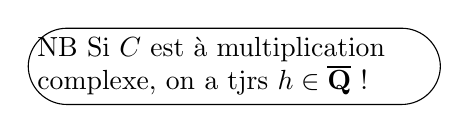
\begin{tikzpicture}\node[draw,rounded corners=14pt,text width=5cm,align=left] {\uline{NB} Si $C$ est à multiplication complexe, on a tjrs $h\in\overline{\mathbf Q}$ !};\end{tikzpicture}}}
\margin{12}
